\section{Sharpness}\label{sec:sharpness}

Let \(\theta^{\ast}\in\reals^{d}\) be a local minimum of \(f\).
The sharpness of the loss landscape at \(\theta^{\ast}\)
quantifies how quickly the loss increases away from \(\theta^{\ast}\).
Intuitive, empirical, and theoretical observations suggest that
sharpness and generalization are linked,
more specifically, sharpness is negatively correlated with generalization
(see \Cref{fig:sharpvflat},~\citealt{keskarLargeBatchTrainingDeep2022}).
\begin{figure}[htb]
	\begin{center}
		% 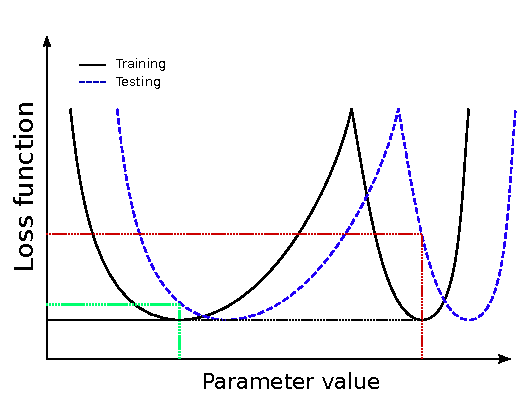
\includegraphics[width=0.6\linewidth]{pdf/sharpvflat}
	\end{center}
	\caption{%
		The flat minimum (left) performs similarly on both training and test data,
		while the sharp minimum (right) performs poorly on test data: it overfits%
		~\cite{keskarLargeBatchTrainingDeep2022}.
	}\label{fig:sharpvflat}
\end{figure}

\subsection{Notions of sharpness}\label{sub:sharpness:notions}

Sharpness, and its converse, flatness,
have been of interest to \gls{abb:ml} researchers for at least since the late 1990s%
~\cite{hochreiterFlatMinima1997}.
Consequently, the community has had time to introduce a panoply
of distinct, yet related notions of sharpness.
In this section we present a non-exhaustive list of such notions,
the interactions therebetween, and the relationship to generalization.

The earliest attempts at quantifying sharpness are based on zeroth-order information
on the function's variation in a neighborhood around a local minimum.
In this vein, \citet{hochreiterFlatMinima1997} introduce
the \(\epsilon\)-flatness (\(\epsilon \gt 0\)) at a local minimum \(\theta^{\ast}\) as
the volume of the largest (for inclusion) connected set \(A \subset \reals^{d}\) such that
\(\theta^{\ast}\in A \) and
\begin{equation}\label{eq:sharpness:epsflatness}
	\forall \theta\in A, \quad f(\theta) \leq f(\theta^{\ast}) + \epsilon.
\end{equation}
Larger volume for smaller \(\epsilon\) indicates a flatter minimum.
\citet{keskarLargeBatchTrainingDeep2022} take the dual perspective,
constraining the volume and using the loss to measure sharpness.
This yields the following definition of what they call \(\epsilon\)-sharpness
\begin{equation}\label{eq:sharpness:epsharpness}
	\max_{\lpnorm[\infty]{\theta - \theta^{\ast}}\le\epsilon}%
	{\frac{f(\theta) - f\left( \theta^{\ast} \right)}{1+f(\theta^{\ast})}}.
\end{equation}
Both of these definitions share a glaring weakness: they cannot handle bounded functions
(see \Cref{fig:epsflat_counterexample}).
\begin{figure}[hbt]
	\begin{center}
		% 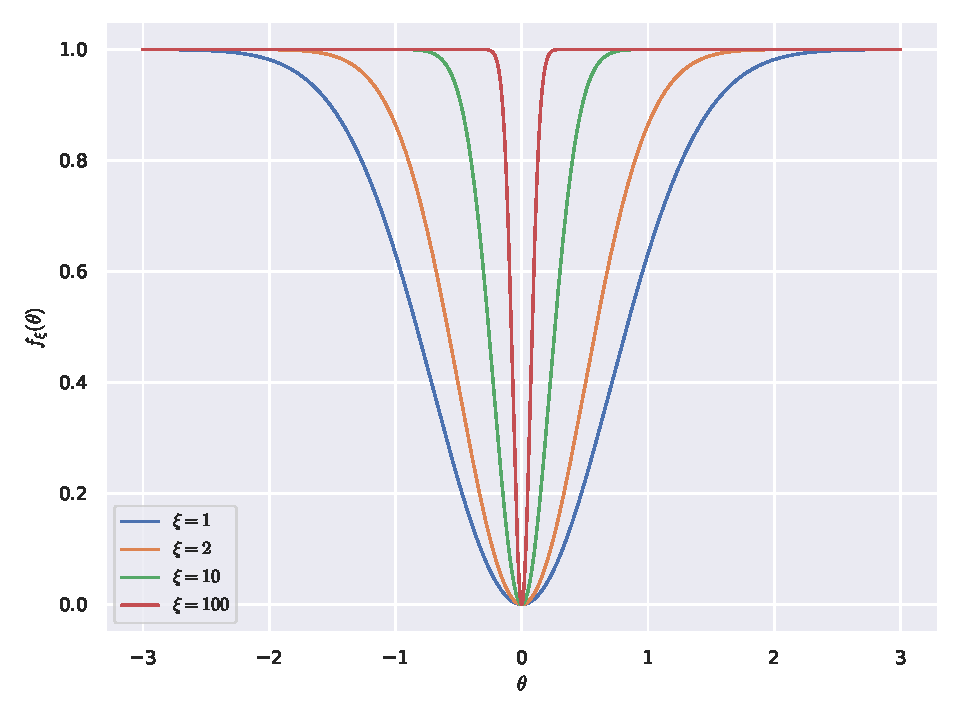
\includegraphics[width=0.6\linewidth]{python/pdf/epsflat_counterexample}
	\end{center}
	\caption{%
		All functions \(f_{\xi}\) are infinitely \(1\)-flat, and \(1\)-sharp at \(\theta^{\ast} = 0\)
		despite looking visually sharper for larger \(\xi\).
	}\label{fig:epsflat_counterexample}
\end{figure}

Other authors resorted to the use of second-order curvature to define sharpness.
Most notably, functions of the spectrum of the loss Hessian matrix
like the trace~\cite{%
	yangTaxonomizingLocalGlobal2021,%
	petzkaRelativeFlatnessGeneralization2021,%
	ibayashiMinimumSharpnessScaleinvariant2021,%
	leeNewCharacterizationEdge2022,%
	petzkaReparameterizationInvariantFlatnessMeasure2019%
}, the spectral norm~\cite{yangTaxonomizingLocalGlobal2021},
and, more generally, the eigenvalue distribution~\cite{%
	keskarLargeBatchTrainingDeep2022,%
	chaudhariEntropySGDBiasingGradient2019%
}.
These measures are not a complete departure from the zeroth-order sharpness measures,
as, for example, \(\epsilon\)-sharpness is approximated by the formula
\[
	\frac{\lambda_{1}\epsilon^{2}}{2 \left( 1+f\left( \theta^{\ast} \right) \right)},
\]
for small \(\epsilon\), where \(\lambda_{1}\) is the maximum eigenvalue of the Hessian
(i.e.,\ the spectral norm)%
~\cite{keskarLargeBatchTrainingDeep2022,zhangWhyFlatnessDoes2021,dinhSharpMinimaCan2017}.
All the metrics introduced so far%
~\cite[including the zeroth-order ones][]{ibayashiMinimumSharpnessScaleinvariant2021}
suffer from a common problem: they are parameter dependent%
~\cite{%
	dinhSharpMinimaCan2017,%
	jangReparametrizationInvariantSharpnessMeasure2022,zhangWhyFlatnessDoes2021,%
	liangFisherRaoMetricGeometry2019%
}.
Sharpness however, is a geometric property, and must be invariant to re-parametrization.

To address this, multiple metrics have been introduced
with invariance to certain classes of transformations.
Relative flatness~\cite{petzkaRelativeFlatnessGeneralization2021}
is one such metric, defined using both parameters and the Hessian,
which is invariant to neuron-wise (and by extension layer-wise) scaling.
Minimum sharpness~\cite{ibayashiMinimumSharpnessScaleinvariant2021}
is similarly invariant to layer-wise scaling.
Defined as the smallest trace of the Hessian over all layer-wise rescalings
that leave the model unchanged, it achieves scale invariance more or less by definition.
The Fisher-Rao norm~\cite{liangFisherRaoMetricGeometry2019},
defined as
\(
\lpnorm[I(\theta^{\ast})]{\theta^{\ast}}^{2} =
\transpose{{\theta^{\ast}}}I(\theta^{\ast})\theta^{\ast}
\),
where \(I(\theta^{\ast})\) is the Fisher information matrix,
is motivated by information geometry and is in fact \emph{intrinsic},
i.e.,\ identical for different parameterizations of the same model.
Pushing this idea further, \citet{jangReparametrizationInvariantSharpnessMeasure2022}
propose another information-geometric sharpness measure,
which is invariant to arbitrary smooth re-parametrizations.
Finally, \citet{zhangWhyFlatnessDoes2021} bypass the issue of parameterization altogether,
by directly defining sharpness in function space.
More concretely, the sharpness of a model is the prior probability that
\gls{abb:sgd} will converge to it from a random initialization.

\begin{enumerate}
	%! Path forward: introduce all of these hessian measures in passing, without much detail,
	%! as it turns outh the Hessian is purely incidental to some of them.
	%! Problem: evrything so far is parameter dependent.
	\item  use Bayesian learning to define in function space.
\end{enumerate}

\subsection{Sharpness and generalization}\label{sub:sharpness:generalization}
\cite{chenBootstrapGeneralizationAbility2023}
Global structure:
\begin{itemize}
	\item \citet{keskarLargeBatchTrainingDeep2022} say that flat minima generalize better than sharp minima.
	\item \citet{%
		      dinhSharpMinimaCan2017,%
		      zhangWhyFlatnessDoes2021,%
		      andriushchenkoModernLookRelationship2023%
	      }
	      question the relationship between sharpness and generalization.
	\item \citet{zhangWhyFlatnessDoes2021} introduce function space sharpness.
	\item \citet{jangReparametrizationInvariantSharpnessMeasure2022}
	      introduce information-geometric sharpness.
\end{itemize}

\cite{%
	andriushchenkoUnderstandingSharpnessAwareMinimization2022,%
	zhangWhyFlatnessDoes2021,%
	tahmasebiUniversalClassSharpnessAware2024,%
	andriushchenkoModernLookRelationship2023,%
	ibayashiMinimumSharpnessScaleinvariant2021,%
	foretSharpnessawareMinimizationEfficiently2020,%
	caldarolaImprovingGeneralizationFederated2022,%
	leeNewCharacterizationEdge2022,%
	chaudhariEntropySGDBiasingGradient2019%
}
